\chapter{二元搜尋樹}
\label{ch:bst}

% 本章的圖共用的樣式（名稱都以 b 開頭，避免和其他章衝突）
\tikzset{
    bnode/.style={circle, draw=black!65, minimum size=7mm, inner sep=0pt, font=\small},
    bnodes/.style={bnode, minimum size=6mm, font=\footnotesize},
    bhl/.style={draw=memStroke, thick, fill=memFill},
    bnew/.style={draw=optStroke, thick, fill=optFill},
    bpath/.style={edge from parent/.style={draw=memStroke, very thick}},
    bst/.style={level distance=10mm, every child node/.style={bnode},
        edge from parent/.style={draw=black!55, thick},
        level 1/.style={sibling distance=48mm},
        level 2/.style={sibling distance=24mm},
        level 3/.style={sibling distance=12mm},
        level 4/.style={sibling distance=7mm}},
    bsts/.style={bst, level distance=9mm, every child node/.style={bnodes},
        level 1/.style={sibling distance=34mm},
        level 2/.style={sibling distance=17mm},
        level 3/.style={sibling distance=8.5mm},
        level 4/.style={sibling distance=6mm}},
    bsize/.style={font=\scriptsize, text=coreStroke, inner sep=1pt},
}

健身房的櫃台用會員編號管理會員，一整天都在做三件事：刷卡時查這個編號是不是有效的
會員，有人入會就加一筆，有人退會就刪一筆。 第~5~章排好的串列，查詢和加入都得從頭
一個一個走；排好的陣列可以二分搜尋，加入一筆卻要把後面的資料全部往後搬。 有沒有一
種存法，讓三件事都只要走大約 $\lg n$ 步？ 提示：回想二分搜尋，每一步其實只看了一個
元素，看完之後就決定往左半邊還是右半邊走。 往下讀之前，先想一想。

把二分搜尋「先看中間、再往左或往右」的結構直接用節點和指標存下來，就是\textbf{二元
搜尋樹}（binary search tree，簡稱 BST）。 每個節點的左邊放比它小的、右邊放比它大
的；查詢從根往下走，每一步往左或往右，插入就是查到空位時接上一個新節點，不用搬動任
何東西。 這一章先講搜尋、最小／最大和前驅／後繼，再講插入和刪除（刪除有三種情況，
每種都畫出來）。 所有操作的成本都和樹高成正比，所以第~\ref{sec:bst-height}~節討論
樹高：最壞會長成一條鏈，隨機的插入順序則讓樹高維持在 $O(\lg n)$ 左右。 最後在每個
節點多記一個「子樹大小」，用它在 $O(h)$ 時間內找第 $k$ 小、算名次。

這一章用到《C 程式設計基礎》第~14~章的結構指標、第~15~章的遞迴、第~19~章的
\texttt{malloc}、指標的指標和 BST 入門（那裡寫過插入和三種走訪，沒有寫刪除），用到
時會先在框裡複習。 樹的名詞和走訪在本書第~7~章，第~5~章的 \texttt{Node **} 寫法這
一章會再用一次。

\section{搜尋、最小／最大、前驅與後繼}
\label{sec:bst-query}

\subsection{定義}

二元搜尋樹是一棵二元樹，每個節點 $x$ 有三個欄位：$x.\mathit{key}$ 是鍵值，
$x.\mathit{left}$、$x.\mathit{right}$ 指向左、右子節點（沒有就是 \NIL）。 樹本身只
記一個指標 $T.\mathit{root}$。 實際的節點還會帶著其他資料（會員姓名、到期日），和
第~5~章一樣，虛擬碼只寫鍵值和指標。 這些節點必須滿足下面的性質。

\begin{definition}[二元搜尋樹性質]
\label{def:bst}
對樹上的每個節點 $x$：$x$ 的左子樹裡\textbf{每一個}節點 $y$ 都有 $y.\mathit{key} <
x.\mathit{key}$，右子樹裡\textbf{每一個}節點 $y$ 都有 $y.\mathit{key} >
x.\mathit{key}$。
\end{definition}

條件是對整棵子樹，只看父子兩個節點不夠。 《C 程式設計基礎》第~19~章有一個反例：
$5$ 的右子節點是 $8$，$8$ 的左子節點是 $4$，每一對父子都沒有排錯，但 $4$ 在 $5$ 的右
子樹裡卻比 $5$ 小。

這一章假設鍵值都不相同，重複的鍵值在插入時忽略，和《C 程式設計基礎》的約定一樣。
真的要存重複的鍵值，常見的做法是在節點裡多記一個「出現次數」，或是把鍵值換成
「鍵值＋序號」這種不會重複的組合（第~\ref{sec:bst-rank}~節的例子會用到）。 有些課
本允許相等的鍵值放在右邊，定義裡的 $>$ 改成 $\ge$；考卷上遇到時，照題目的規定。

\textbf{深度}和\textbf{高度}照第~7~章的定義：深度數邊，根的深度是 $0$，節點的深度是
它到根的路徑上有幾條邊；高度數節點，樹高 $h$ 是樹的層數，也就是最大深度加 $1$。 只有
一個節點的樹高度是 $1$，空樹的高度是 $0$。 CLRS 的高度數邊，算出來會比這裡少 $1$。

下面是本章前兩節一直用的例子：依序加入 $52,\allowbreak 27,\allowbreak 74,\allowbreak 15,\allowbreak 40,\allowbreak 63,\allowbreak 88,\allowbreak 33,\allowbreak 46,\allowbreak 58,\allowbreak 70,\allowbreak 95,\allowbreak 36$ 這 $13$ 位會員（編號只寫末兩碼），得到的樹。 第~\ref{sec:bst-modify}~節會一
步一步插入；這裡先看結果。

\begin{center}
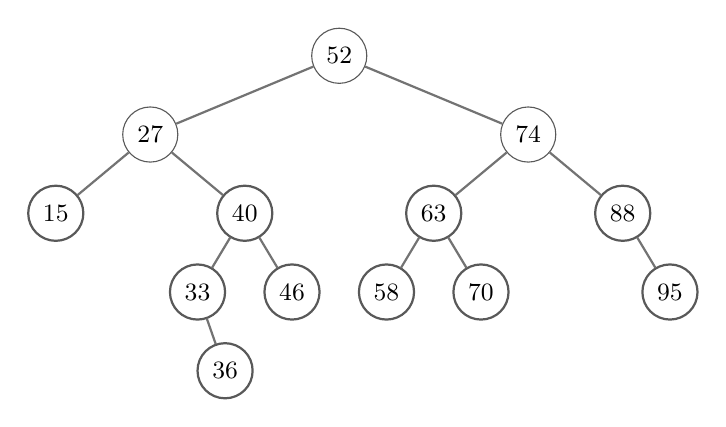
\begin{tikzpicture}[bst]
\node[bnode] {52}
  child {node {27}
    child {node {15}}
    child {node {40}
      child {node {33}
        child[missing]
        child {node {36}}}
      child {node {46}}}}
  child {node {74}
    child {node {63}
      child {node {58}}
      child {node {70}}}
    child {node {88}
      child[missing]
      child {node {95}}}};
\end{tikzpicture}
\diagcaption{$13$ 個會員編號組成的二元搜尋樹 $T$，高度 $5$（最深的是 $36$，深度 $4$）。 根
$52$ 的左子樹都比 $52$ 小，右子樹都比 $52$ 大；每一棵子樹也都是這樣。}
\label{fig:bst-T}
\end{center}

對一棵二元搜尋樹做第~7~章的\textbf{中序走訪}（先左子樹、再自己、再右子樹），會由
小到大印出所有鍵值。 在圖~\ref{fig:bst-T} 上是 $15,\allowbreak 27,\allowbreak 33,\allowbreak 36,\allowbreak 40,\allowbreak 46,\allowbreak 52,\allowbreak 58,\allowbreak 63,\allowbreak 70,\allowbreak 74,\allowbreak 88,\allowbreak 95$。

\begin{theorem}
\label{thm:bst-inorder}
對二元搜尋樹做中序走訪，印出的鍵值由小到大排列。 $n$ 個節點時走訪的時間是
$\Theta(n)$。
\end{theorem}

\begin{proof}
對子樹的節點數做歸納。 空樹什麼都不印，成立。 設根是 $x$，左、右子樹的節點數都比整
棵少，由歸納假設，走訪左子樹印出的是左子樹的鍵值，由小到大；右子樹也是。 由
定義~\ref{def:bst}，左子樹的鍵值都比 $x.\mathit{key}$ 小，右子樹的都比它大，所以
「左子樹的遞增序列、$x.\mathit{key}$、右子樹的遞增序列」接起來仍然遞增。 時間：每
個節點印一次，每個 \NIL 子樹各花常數時間，而 $n$ 個節點的二元樹恰好有 $n + 1$ 個
\NIL 子樹（第~7~章），合計 $\Theta(n)$。
\end{proof}

反過來也成立：一棵二元樹的中序走訪如果是遞增的，它就是二元搜尋樹。 所以「檢查一棵
樹是不是 BST」可以只做一次中序走訪，看每個鍵值是否比前一個大。

\subsection{搜尋}

二元搜尋樹和二分搜尋的關係，看下面這張圖最清楚。 對排好的陣列 $15,\allowbreak 27,\allowbreak 33,\allowbreak 40,\allowbreak 52,\allowbreak 63,\allowbreak 74$ 做二分搜尋，第一步一定看中間的 $40$；比 $40$ 小就到左半邊 $15, 27, 33$，
看它的中間 $27$；比 $40$ 大就看右半邊的中間 $63$。 把「每一步可能看的元素」畫出來，
就是一棵二元搜尋樹。

\begin{center}
\begin{tikzpicture}
\foreach \v [count=\k] in {15, 27, 33, 40, 52, 63, 74} {
    \node[cell] (a\k) at (\k*0.9, 0) {\v};
}
\node[idxlbl, anchor=east] at (0.3, 0) {陣列};
\begin{scope}[xshift=10.6cm, yshift=0.6cm, bsts]
\node[bnodes] {40}
  child {node {27} child {node {15}} child {node {33}}}
  child {node {63} child {node {52}} child {node {74}}};
\end{scope}
\draw[diagarrow] (7.0, 0) -- (8.2, 0);
\end{tikzpicture}
\diagcaption{二分搜尋每一步看的元素排成一棵樹。 陣列可以用位址算出中間那一格；
樹把「中間是誰」直接存成指標，所以插入新元素時不必搬動其他元素。}
\label{fig:bst-binsearch}
\end{center}

搜尋鍵值 $k$ 時，從根開始和 $x.\mathit{key}$ 比較：相等就找到了；$k$ 比較小，答案只
可能在左子樹，往左走；比較大就往右走。 走到 \NIL 表示 $k$ 不在樹裡。

\begin{pseudo}[label=alg:bst-search]{在以 $x$ 為根的子樹裡找 $k$（遞迴）}
\Function{Tree-Search}{$x, k$}
    \If{$x = \NIL$ \OR $k = x.\mathit{key}$}
        \State \Return $x$
    \EndIf
    \If{$k < x.\mathit{key}$}
        \State \Return \Call{Tree-Search}{$x.\mathit{left}, k$}
    \Else
        \State \Return \Call{Tree-Search}{$x.\mathit{right}, k$}
    \EndIf
\EndFunction
\end{pseudo}

呼叫的方式是 \proc{Tree-Search}$(T.\mathit{root}, k)$。 每一層遞迴只往下走一步，而且
遞迴呼叫是函式的最後一個動作，可以直接改成迴圈，省掉呼叫堆疊（第~6~章）：

\begin{pseudo}[label=alg:bst-search-iter]{在以 $x$ 為根的子樹裡找 $k$（迴圈）}
\Function{Iterative-Tree-Search}{$x, k$}
    \While{$x \ne \NIL$ \AND $k \ne x.\mathit{key}$}
        \If{$k < x.\mathit{key}$}
            \State $x \gets x.\mathit{left}$
        \Else
            \State $x \gets x.\mathit{right}$
        \EndIf
    \EndWhile
    \State \Return $x$
\EndFunction
\end{pseudo}

兩個版本走過的節點完全一樣，都在一條從根往下的路徑上，每層最多一個，所以最多比較
$h$ 個節點，時間 $O(h)$，$h$ 是樹高。 下表是在圖~\ref{fig:bst-T} 上搜尋 $46$ 和 $60$ 的過程。

\begin{center}
\begin{tabular}{cccl}
\toprule
搜尋 & 第幾次比較 & $x.\mathit{key}$ & 結果 \\
\midrule
$46$ & 1 & 52 & $46 < 52$，往左 \\
     & 2 & 27 & $46 > 27$，往右 \\
     & 3 & 40 & $46 > 40$，往右 \\
     & 4 & 46 & 相等，找到 \\
\midrule
$60$ & 1 & 52 & $60 > 52$，往右 \\
     & 2 & 74 & $60 < 74$，往左 \\
     & 3 & 63 & $60 < 63$，往左 \\
     & 4 & 58 & $60 > 58$，往右，$x = \NIL$，找不到 \\
\bottomrule
\end{tabular}
\end{center}

找不到 $60$ 時，最後停在 $58$ 的右邊。 這個空位剛好就是插入 $60$ 時新節點要接的地
方，第~\ref{sec:bst-modify}~節的插入就是利用這件事。

\subsection{最小與最大}

最小的鍵值在哪裡？ 從根一直往左走，走到沒有左子節點為止。 理由：如果 $x$ 有左子節
點，左子樹裡的鍵值都比 $x$ 小，最小值一定不是 $x$，也不在 $x$ 的右子樹，只能在左子
樹；如果 $x$ 沒有左子節點，子樹裡其他的鍵值都在右邊，都比 $x$ 大，所以 $x$ 就是最
小值。 最大值左右對調。

\begin{pseudo}[label=alg:bst-minmax]{以 $x$ 為根的子樹裡的最小值、最大值（$x \ne \NIL$）}
\Function{Tree-Minimum}{$x$}
    \While{$x.\mathit{left} \ne \NIL$}
        \State $x \gets x.\mathit{left}$
    \EndWhile
    \State \Return $x$
\EndFunction
\Function{Tree-Maximum}{$x$}
    \While{$x.\mathit{right} \ne \NIL$}
        \State $x \gets x.\mathit{right}$
    \EndWhile
    \State \Return $x$
\EndFunction
\end{pseudo}

圖~\ref{fig:bst-T} 的最小值是 $52 \to 27 \to 15$，最大值是 $52 \to 74 \to 88 \to
95$。 注意最大值 $95$ 剛好是葉節點，但這不是必然的：最小值所在的節點一定沒有左子節
點，卻可能有右子節點。 例如刪掉 $15$ 之後，最小值變成 $27$，它有右子樹。 時間一樣
是 $O(h)$。

\subsection{後繼與前驅}

節點 $x$ 的\textbf{後繼}（successor）是中序走訪裡排在 $x$ 下一個的節點，也就是鍵值
比 $x.\mathit{key}$ 大的節點裡最小的那個；\textbf{前驅}（predecessor）是排在前一個
的節點。 $x$ 是最大值時沒有後繼，回傳 \NIL。 刪除（下一節）和第 $k$ 小的應用都需要
它。

找後繼分兩種情況。

\begin{enumerate}
\item \textbf{$x$ 有右子樹。} 右子樹的鍵值都比 $x$ 大；樹上其他比 $x$ 大的鍵值，如果
在 $x$ 的某個祖先 $y$ 那裡，那是因為 $x$ 在 $y$ 的左子樹裡，這時 $x$ 的右子樹也整棵
在 $y$ 的左子樹裡，都比 $y$ 小。 所以後繼是右子樹的最小值。 圖~\ref{fig:bst-T} 裡
$27$ 的後繼是右子樹 $\{40, 33, 36, 46\}$ 的最小值 $33$。
\item \textbf{$x$ 沒有右子樹。} 後繼一定是 $x$ 的祖先。 從 $x$ 往上走，只要目前的節
點是父節點的右子節點，父節點就比它小，繼續往上；第一次「從左邊走上來」時，那個父
節點就是後繼。 圖~\ref{fig:bst-T} 裡 $46$ 是 $40$ 的右子節點，$40$ 是 $27$ 的右子節
點，$27$ 是 $52$ 的左子節點，所以 $46$ 的後繼是 $52$。 走到根都沒有從左邊上來，表
示 $x$ 是最大值。
\end{enumerate}

\begin{center}
\begin{tikzpicture}[bst]
\node[bnode, bhl] {52}
  child[bpath] {node[bhl] {27}
    child[black!55] {node {15}}
    child[bpath] {node[bhl] {40}
      child {node {33}
        child[missing]
        child {node {36}}}
      child[bpath] {node[bnew] {46}}}}
  child {node {74}
    child {node {63}
      child {node {58}}
      child {node {70}}}
    child {node {88}
      child[missing]
      child {node {95}}}};
\node[font=\scriptsize, text=memStroke, anchor=west] at (0.5, 0) {後繼};
\end{tikzpicture}
\diagcaption{$46$ 沒有右子樹，往上走：$46 \to 40$、$40 \to 27$ 都是從右邊上去；
$27 \to 52$ 是從左邊上去，所以 $46$ 的後繼是 $52$。}
\label{fig:bst-succ}
\end{center}

第二種情況要能從節點往上走，所以節點要多一個欄位 $x.p$ 指向父節點（根的 $p$ 是
\NIL）。 有 $p$ 的寫法如下：

\begin{pseudo}[label=alg:bst-succ]{節點 $x$ 的後繼（節點有父指標 $p$）}
\Function{Tree-Successor}{$x$}
    \If{$x.\mathit{right} \ne \NIL$}
        \State \Return \Call{Tree-Minimum}{$x.\mathit{right}$}
    \EndIf
    \State $y \gets x.p$
    \While{$y \ne \NIL$ \AND $x = y.\mathit{right}$} \Comment{從右邊上來，繼續}
        \State $x \gets y$
        \State $y \gets y.p$
    \EndWhile
    \State \Return $y$
\EndFunction
\end{pseudo}

不想多存父指標，也可以從根往下找。 從根往下走向 $x.\mathit{key}$ 的路上，每次往左
轉，那個節點就比 $x.\mathit{key}$ 大，是後繼的候選；越晚往左轉的候選越小。 所以只要
記住「最後一次往左轉的節點」。 走到 $x$ 之後，如果 $x$ 有右子樹，就照同樣的規則繼
續走進右子樹：右子樹的鍵值都比 $x.\mathit{key}$ 大，先往右一步，接著一路往左，每一
步都更新候選，最後停在右子樹的最小值。 兩種情況因此可以寫成同一個迴圈：

\begin{pseudo}[label=alg:bst-succ-key]{比 $k$ 大的最小鍵值（不用父指標）}
\Function{Successor-Of-Key}{$T, k$}
    \State $s \gets \NIL$ \Comment{目前看到比 $k$ 大的最小節點}
    \State $x \gets T.\mathit{root}$
    \While{$x \ne \NIL$}
        \If{$k < x.\mathit{key}$}
            \State $s \gets x$
            \State $x \gets x.\mathit{left}$
        \Else
            \State $x \gets x.\mathit{right}$
        \EndIf
    \EndWhile
    \State \Return $s$
\EndFunction
\end{pseudo}

這個版本還有一個好處：$k$ 不必在樹裡。 例如 $k = 60$ 時它回傳 $63$，回答的是「編號
$60$ 之後的下一位會員是誰」。 下表是 $k = 46$ 和 $k = 27$ 的過程。

\begin{center}
\begin{tabular}{ccccc}
\toprule
$k$ & $x.\mathit{key}$ & 比較 & 動作 & $s$ \\
\midrule
$46$ & 52 & $46 < 52$ & $s \gets 52$，往左 & 52 \\
     & 27 & $46 \ge 27$ & 往右 & 52 \\
     & 40 & $46 \ge 40$ & 往右 & 52 \\
     & 46 & $46 \ge 46$ & 往右，$x = \NIL$ & 52 \\
\midrule
$27$ & 52 & $27 < 52$ & $s \gets 52$，往左 & 52 \\
     & 27 & $27 \ge 27$ & 往右 & 52 \\
     & 40 & $27 < 40$ & $s \gets 40$，往左 & 40 \\
     & 33 & $27 < 33$ & $s \gets 33$，往左，$x = \NIL$ & 33 \\
\bottomrule
\end{tabular}
\end{center}

兩個版本都只沿著一條路徑往上或往下走，時間 $O(h)$。 前驅把左右對調：有左子樹就是左
子樹的最大值，否則往上找第一個「從右邊走上來」的祖先；不用父指標的版本則改成記住最後
一次往右轉的節點。 圖~\ref{fig:bst-T} 裡 $58$ 沒有左子樹，往上 $58 \to 63 \to 74$
都是從左邊上去，$74 \to 52$ 是從右邊上去，所以 $58$ 的前驅是 $52$。

\begin{examnote}
追蹤搜尋、後繼、前驅時，把走過的節點依序寫成一列，例如「$52 \to 27 \to 40 \to 46$，
找到」，每一步旁邊註明比較的結果。 求後繼時先寫「$x$ 有沒有右子樹」，再寫用哪一種情
況。 題目給的樹如果沒有說節點有父指標，就用從根往下的寫法，不要假設可以往上走。
\end{examnote}

\section{插入、刪除}
\label{sec:bst-modify}

\subsection{插入}

插入新節點 $z$ 的方法就是先搜尋 $z.\mathit{key}$：搜尋失敗時停下的那個 \NIL，就是
$z$ 的位置。 走的時候讓 $y$ 跟在 $x$ 後面一層，$x$ 變成 \NIL 時，$y$ 就是 $z$ 的父節
點，再看 $z.\mathit{key}$ 比 $y.\mathit{key}$ 小還是大，決定接在左邊還是右邊。 這和
第~5~章依序插入串列時讓 $p$ 跟在 $q$ 後面是同一個做法。

\begin{pseudo}[label=alg:bst-insert]{插入節點 $z$（$z.\mathit{left} = z.\mathit{right} = \NIL$，鍵值不在樹裡）}
\Procedure{Tree-Insert}{$T, z$}
    \State $y \gets \NIL$ \Comment{$y$ 跟在 $x$ 後面一層}
    \State $x \gets T.\mathit{root}$
    \While{$x \ne \NIL$}
        \State $y \gets x$
        \If{$z.\mathit{key} < x.\mathit{key}$}
            \State $x \gets x.\mathit{left}$
        \Else
            \State $x \gets x.\mathit{right}$
        \EndIf
    \EndWhile
    \If{$y = \NIL$}
        \State $T.\mathit{root} \gets z$ \Comment{樹原本是空的}
    \ElsIf{$z.\mathit{key} < y.\mathit{key}$}
        \State $y.\mathit{left} \gets z$
    \Else
        \State $y.\mathit{right} \gets z$
    \EndIf
\EndProcedure
\end{pseudo}

新節點永遠接成葉節點，原本的節點一個都不動，所以插入之後樹仍然滿足
定義~\ref{def:bst}：$z$ 走過的每個節點，$z$ 都放在正確的那一邊。 走過的節點最多
$h$ 個（$h$ 是插入前的樹高），時間 $O(h)$。 節點有父指標時，在第 10 行之前加一行 $z.p \gets y$。

第~\ref{sec:bst-query}~節的例子就是對空樹依序插入 $52,\allowbreak 27,\allowbreak 74,\allowbreak 15,\allowbreak 40,\allowbreak 63,\allowbreak 88,\allowbreak 33,\allowbreak 46,\allowbreak 58,\allowbreak 70,\allowbreak 95,\allowbreak 36$。 考卷上常要求寫出每一次插入的比較過程，下表一列寫一個鍵值。

\begin{center}
\begin{tabular}{cll}
\toprule
插入 & 比較過的節點 & 接在 \\
\midrule
52 & （空樹） & 成為根 \\
27 & 52 & 52 的左邊 \\
74 & 52 & 52 的右邊 \\
15 & 52, 27 & 27 的左邊 \\
40 & 52, 27 & 27 的右邊 \\
63 & 52, 74 & 74 的左邊 \\
88 & 52, 74 & 74 的右邊 \\
33 & 52, 27, 40 & 40 的左邊 \\
46 & 52, 27, 40 & 40 的右邊 \\
58 & 52, 74, 63 & 63 的左邊 \\
70 & 52, 74, 63 & 63 的右邊 \\
95 & 52, 74, 88 & 88 的右邊 \\
36 & 52, 27, 40, 33 & 33 的右邊 \\
\bottomrule
\end{tabular}
\end{center}

一個鍵值插入時比較了幾個節點，就等於它的深度。 把這一欄加起來，就是建這棵樹總共比
較的次數：$0 + 1 + 1 + 2 + 2 + 2 + 2 + 3 + 3 + 3 + 3 + 3 + 4 = 29$。 樹的形狀完全由
插入順序決定。 同樣這 $13$ 個編號，如果由小到大插入，每個新節點都接在前一個的右
邊，樹會變成一條鏈，第~\ref{sec:bst-height}~節再回來看這件事。

\subsection{刪除的三種情況}

刪除節點 $z$ 比插入麻煩，因為 $z$ 可能在樹的中間，拿掉它之後兩棵子樹要有人接手。 依
$z$ 有幾個子節點分成三種情況。

\begin{enumerate}
\item \textbf{$z$ 沒有子節點（葉節點）。} 直接拿掉，父節點指向 $z$ 的那個指標改成
\NIL。
\item \textbf{$z$ 只有一個子節點。} 讓這個子節點連同它的子樹頂上來，接在 $z$ 原本的
位置。 這樣做仍然是 BST：那棵子樹原本就在 $z$ 的父節點的同一邊。
\item \textbf{$z$ 有兩個子節點。} 找 $z$ 的後繼 $s$，也就是右子樹的最小值，用 $s$ 取
代 $z$。 $s$ 比左子樹的每個鍵值大（因為它比 $z$ 大），又比右子樹裡其他的鍵值小（因為
它是右子樹的最小值），放在 $z$ 的位置剛好。 $s$ 是右子樹的最小值，所以\textbf{沒有左
子節點}，把它從原位拿掉時屬於情況 1 或 2，不會再遇到兩個子節點。
\end{enumerate}

情況 3 也可以用前驅（左子樹的最大值）取代 $z$，理由左右對調，前驅一定沒有右子節
點。 兩種都是對的，但結果的樹不一樣；本書沒有特別說明時都用後繼。

下面用圖~\ref{fig:bst-T} 依序刪除 $46$、$88$、$27$、$74$，四種狀況各遇到一次。

\begin{enumerate}
\item 刪除 $46$：葉節點，$40$ 的右子節點改成 \NIL。
\item 刪除 $88$：只有右子節點 $95$，$95$ 頂上來成為 $74$ 的右子節點。
\item 刪除 $27$：兩個子節點。 後繼是右子樹 $\{40, 33, 36\}$ 的最小值 $33$，它在右子
樹的深處，而且有右子節點 $36$。 先把 $33$ 從原位拿掉（情況 2：$36$ 頂上來成為
$40$ 的左子節點），再讓 $33$ 坐到 $27$ 的位置，接手 $27$ 的左子樹 $15$ 和右子樹
$40$。
\item 刪除 $74$：兩個子節點。 這時 $74$ 的右子樹只剩 $95$，後繼 $95$ 就是 $74$ 的右子
節點本身。 $95$ 沒有左子節點，直接坐到 $74$ 的位置，接手左子樹 $63$，右邊是它原本的
右子樹（空的）。
\end{enumerate}

\begin{center}
\begin{minipage}{0.49\linewidth}\centering
\begin{tikzpicture}[bsts]
\node[bnodes] {52}
  child {node {27}
    child {node {15}}
    child {node {40}
      child {node {33}
        child[missing]
        child {node {36}}}
      child[missing]}}
  child {node {74}
    child {node {63}
      child {node {58}}
      child {node {70}}}
    child {node[bhl] {88}
      child[missing]
      child {node {95}}}};
\end{tikzpicture}

{\footnotesize (a) 刪除 $46$ 之後；下一步刪 $88$}
\end{minipage}\hfill
\begin{minipage}{0.49\linewidth}\centering
\begin{tikzpicture}[bsts]
\node[bnodes] {52}
  child {node[bhl] {27}
    child {node {15}}
    child {node {40}
      child {node[bnew] {33}
        child[missing]
        child {node {36}}}
      child[missing]}}
  child {node {74}
    child {node {63}
      child {node {58}}
      child {node {70}}}
    child {node {95}}};
\end{tikzpicture}

{\footnotesize (b) 刪除 $88$ 之後；下一步刪 $27$，後繼是 $33$}
\end{minipage}

\medskip
\begin{minipage}{0.49\linewidth}\centering
\begin{tikzpicture}[bsts]
\node[bnodes] {52}
  child {node {33}
    child {node {15}}
    child {node {40}
      child {node {36}}
      child[missing]}}
  child {node[bhl] {74}
    child {node {63}
      child {node {58}}
      child {node {70}}}
    child {node[bnew] {95}}};
\end{tikzpicture}

{\footnotesize (c) 刪除 $27$ 之後；下一步刪 $74$，後繼是 $95$}
\end{minipage}\hfill
\begin{minipage}{0.49\linewidth}\centering
\begin{tikzpicture}[bsts]
\node[bnodes] {52}
  child {node {33}
    child {node {15}}
    child {node {40}
      child {node {36}}
      child[missing]}}
  child {node[bnew] {95}
    child {node {63}
      child {node {58}}
      child {node {70}}}
    child[missing]};
\end{tikzpicture}

{\footnotesize (d) 刪除 $74$ 之後}
\end{minipage}
\diagcaption{從圖~\ref{fig:bst-T} 依序刪除 $46$、$88$、$27$、$74$。 橘色是下一步要刪
的節點，粉紅色是用來取代它的後繼。 (b) 到 (c) 時，$33$ 先離開原位（$36$ 頂上去），
再坐到 $27$ 的位置；(c) 到 (d) 時，後繼 $95$ 就是 $74$ 的右子節點。}
\label{fig:bst-delete}
\end{center}

\subsection{刪除的虛擬碼}

情況 3 有兩種常見的寫法。 第一種把後繼 $s$ 的鍵值（連同其他資料）複製到 $z$ 裡，再到
右子樹裡刪掉 $s$；節點 $z$ 留在原地，換掉的是它存的東西。 第二種不複製資料，改接指
標，把節點 $s$ 本身搬到 $z$ 的位置。 兩種寫法刪除之後，每個位置上的鍵值完全一樣，畫
出來的樹相同。 差別在節點：如果程式的其他地方存著指向某個節點的指標（例如「目前選取
的會員」），複製的寫法會讓 $s$ 的資料搬到另一個節點去，那些指標就指錯了。

虛擬碼用第一種，寫成遞迴：函式回傳刪除之後這棵子樹的根，呼叫的人把它接回去。 這
和《C 程式設計基礎》第~19~章遞迴插入的寫法一樣，呼叫方式是 $T.\mathit{root} \gets
\proc{Tree-Delete}(T.\mathit{root}, k)$。

\begin{pseudo}[label=alg:bst-delete]{刪除鍵值 $k$，回傳子樹新的根}
\Function{Tree-Delete}{$x, k$}
    \If{$x = \NIL$}
        \State \Return \NIL \Comment{$k$ 不在樹裡}
    \EndIf
    \If{$k < x.\mathit{key}$}
        \State $x.\mathit{left} \gets \Call{Tree-Delete}{x.\mathit{left}, k}$
    \ElsIf{$k > x.\mathit{key}$}
        \State $x.\mathit{right} \gets \Call{Tree-Delete}{x.\mathit{right}, k}$
    \ElsIf{$x.\mathit{left} = \NIL$} \Comment{情況 1、2：沒有左子節點}
        \State \Return $x.\mathit{right}$
    \ElsIf{$x.\mathit{right} = \NIL$} \Comment{情況 2：只有左子節點}
        \State \Return $x.\mathit{left}$
    \Else \Comment{情況 3：兩個子節點}
        \State $s \gets \Call{Tree-Minimum}{x.\mathit{right}}$
        \State $x.\mathit{key} \gets s.\mathit{key}$ \Comment{連同其他資料一起複製}
        \State $x.\mathit{right} \gets \Call{Tree-Delete}{x.\mathit{right}, s.\mathit{key}}$
    \EndIf
    \State \Return $x$
\EndFunction
\end{pseudo}

第 8 行同時處理了情況 1 和「只有右子節點」的情況 2：沒有左子節點時，右子樹（可能是
空的）頂上來。 第 15 行到右子樹裡刪 $s.\mathit{key}$，那一次遞迴會停在 $s$，而 $s$ 沒
有左子節點，走第 9 行，不會再進入情況 3。 被拿掉的節點（第 9、11 行回傳之後的 $x$）
由呼叫的程式釋放。

時間：第 4 到 7 行沿著一條路徑往下找 $k$；找到之後，情況 3 再從 $x$ 往下走到 $s$，
第 15 行的遞迴走的也是這一段路。 全部都在從根往下的一條路徑上，時間 $O(h)$。

\begin{cbookrecap}[第~14~章、第~15~章、第~19~章 19.10、19.11、19.15 節]
\texttt{x->left} 是 \texttt{(*x).left}。 遞迴函式回傳「更新後的子樹根」時，呼叫
端一定要寫 \texttt{x->left = f(x->left, ...)} 把它接回去；只呼叫不接，子樹的改變
會遺失。

\texttt{Node **link} 存的是「某個 \texttt{Node *} 變數的位址」，可能是根指標
\texttt{root}，也可能是某個節點的 \texttt{left} 或 \texttt{right} 欄位。 寫
\texttt{*link = q} 就把那個指標改成指向 \texttt{q}，不必知道它是根還是哪個節點的
哪一邊。 第~19~章用它寫串列的刪除，本書第~5~章用它寫依序插入；這一節把同樣的寫法
用在樹上。
\end{cbookrecap}

\subsection{C 實作}

C 版用第二種寫法（接指標，不複製資料），而且不用遞迴，也不存父指標。 關鍵是
\texttt{find\_link}：從 \texttt{root} 往下找 \texttt{key}，回傳「指向那個節點的指標
欄位」的位址。 找不到時，回傳的欄位是 \texttt{NULL}，正好是插入時要接的空位，所以插
入和刪除共用它。 刪除情況 3 時，再用一個 \texttt{slink} 從 \texttt{\&z->right} 一路往
左找到「指向後繼 \texttt{s} 的欄位」，先 \texttt{*slink = s->right} 把 $s$ 拿下來，
再讓 $s$ 接手 $z$ 的兩棵子樹。

程式依序插入那 $13$ 個編號，查幾個編號在不在、下一位是誰（\proc{Successor-Of-Key}
的 C 版），再依序刪除 $46$、$88$、$27$、$74$。 \texttt{show} 印出樹的形狀，格式是
「鍵值(左子樹,右子樹)」，空的子樹印 \texttt{-}，葉節點只印鍵值，可以對照
圖~\ref{fig:bst-T} 和圖~\ref{fig:bst-delete}。

\begin{example}[label=ex:bst-member]{c}{(member\_tree.c) 會員編號的二元搜尋樹}
#include <stdio.h>
#include <stdlib.h>

typedef struct Node {
    int key;                    // 會員編號（這裡只用末兩碼）
    struct Node *left, *right;
} Node;

// 回傳「指向 key 所在節點」的那個指標欄位的位址。key 不在樹裡時，
// 那個欄位是 NULL，正好是 key 應該插入的空位。
Node **find_link(Node **root, int key)
{
    Node **link = root;
    while (*link != NULL && (*link)->key != key)
        link = key < (*link)->key ? &(*link)->left : &(*link)->right;
    return link;
}

// 成功回傳 1，已經在樹裡回傳 0，要不到記憶體回傳 -1。
int insert(Node **root, int key)
{
    Node **link = find_link(root, key);
    if (*link != NULL)
        return 0;
    Node *z = malloc(sizeof *z);
    if (z == NULL)
        return -1;
    z->key = key;
    z->left = z->right = NULL;
    *link = z;                  // 接在找到的空位上
    return 1;
}

// 比 key 大的最小鍵值所在的節點；沒有就回傳 NULL。
const Node *successor(const Node *x, int key)
{
    const Node *best = NULL;
    while (x != NULL) {
        if (key < x->key) {
            best = x;           // 往左轉：x 是目前的候選
            x = x->left;
        } else {
            x = x->right;
        }
    }
    return best;
}

// 刪除 key。成功回傳 1，找不到回傳 0。
int erase(Node **root, int key)
{
    Node **link = find_link(root, key);
    Node *z = *link;
    if (z == NULL)
        return 0;
    if (z->left == NULL) {              // 沒有左子：右子樹頂上來
        *link = z->right;
    } else if (z->right == NULL) {      // 只有左子：左子樹頂上來
        *link = z->left;
    } else {                            // 兩個子節點：用後繼 s 取代 z
        Node **slink = &z->right;
        while ((*slink)->left != NULL)
            slink = &(*slink)->left;
        Node *s = *slink;
        *slink = s->right;              // 先把 s 從原位拿掉
        s->left = z->left;              // 再讓 s 接手 z 的兩棵子樹
        s->right = z->right;
        *link = s;
    }
    free(z);
    return 1;
}

// 印出樹的形狀：鍵值(左子樹,右子樹)；空的子樹印 -，葉節點只印鍵值。
void show(const Node *x)
{
    if (x == NULL) {
        putchar('-');
        return;
    }
    printf("%d", x->key);
    if (x->left != NULL || x->right != NULL) {
        putchar('(');
        show(x->left);
        putchar(',');
        show(x->right);
        putchar(')');
    }
}

void free_tree(Node *x)         // 後序：先釋放兩棵子樹，再釋放自己
{
    if (x == NULL)
        return;
    free_tree(x->left);
    free_tree(x->right);
    free(x);
}

int main(void)
{
    Node *root = NULL;
    int join[] = {52, 27, 74, 15, 40, 63, 88, 33, 46, 58, 70, 95, 36};
    int ask[] = {46, 27, 60, 95}, quit[] = {46, 88, 27, 74};
    for (int i = 0; i < 13; i++)
        if (insert(&root, join[i]) < 0)
            break;
    show(root);
    printf("\n");
    for (int i = 0; i < 4; i++) {
        const Node *s = successor(root, ask[i]);
        printf("%d %s, next ", ask[i],
               *find_link(&root, ask[i]) != NULL ? "found" : "missing");
        if (s != NULL)
            printf("%d\n", s->key);
        else
            printf("none\n");
    }
    for (int i = 0; i < 4; i++) {
        erase(&root, quit[i]);
        printf("erase %d: ", quit[i]);
        show(root);
        printf("\n");
    }
    free_tree(root);
    return 0;
}
\end{example}
\iosample{}{52(27(15,40(33(-,36),46)),74(63(58,70),88(-,95))) \\ 46 found, next 52 \\ 27 found, next 33 \\ 60 missing, next 63 \\ 95 found, next none \\ erase 46: 52(27(15,40(33(-,36),-)),74(63(58,70),88(-,95))) \\ erase 88: 52(27(15,40(33(-,36),-)),74(63(58,70),95)) \\ erase 27: 52(33(15,40(36,-)),74(63(58,70),95)) \\ erase 74: 52(33(15,40(36,-)),95(63(58,70),-))}

程式有三個地方要說明：

\begin{itemize}
\item \texttt{erase} 的前兩個分支對應虛擬碼的第 8 到 11 行，\texttt{*link} 可能是
\texttt{root} 本身，所以刪根的時候也不用另外處理。
\item 情況 3 的兩個子情況（後繼在深處、後繼就是右子節點）用的是同一段程式。 刪除
$74$ 時，\texttt{slink} 一開始就是 \texttt{\&z->right}，迴圈一次都沒跑；
\texttt{*slink = s->right} 讓 \texttt{z->right} 變成 \texttt{s} 的右子樹（空的），下
一行 \texttt{s->right = z->right} 讀到的就是這個新值，結果仍然正確。 可以對照圖
~\ref{fig:bst-delete} 的 (c)、(d) 自己走一次。
\item 釋放整棵樹要用後序，先釋放兩棵子樹，最後才釋放自己；用前序的話，
\texttt{free(x)} 之後還要讀 \texttt{x->left}。 \texttt{show} 和 \texttt{free\_tree}
的遞迴深度等於樹高，樹長成一條鏈時會到 $n$；搜尋、插入、刪除都用迴圈，沒有這個問
題。
\end{itemize}

\begin{examnote}
刪除題先判斷節點有幾個子節點，寫出是哪一種情況；兩個子節點時寫出用的是後繼還是前
驅，以及它是誰。 題目沒有指定時，選一種並寫明，整題都用同一種。 答案畫完整棵樹，不
要只畫改到的那一塊，最後用中序走訪檢查一次是否仍然遞增。
\end{examnote}

\section{高度：最壞情況與隨機插入}
\label{sec:bst-height}

前兩節的每個操作都沿著一條從根往下的路徑走，時間都是 $O(h)$。 所以 BST 快不快，全看
樹高 $h$。

\subsection{最好與最壞}

$n$ 個節點的二元樹，高度最少是 $\lceil \lg(n + 1) \rceil$，最多是 $n$（第~7~章）。
兩個極端都會出現在 BST 上。 鍵值由小到大插入時，每個新鍵值都比樹上所有的大，從根一
路往右走到底，接在最右邊，樹變成一條往右的鏈，高度 $n$；由大到小插入是往左的
鏈。 這時 BST 和排好的串列一樣，搜尋要 $\Theta(n)$，依序插入 $n$ 個鍵值總共比較
\[
0 + 1 + 2 + \cdots + (n - 1) = \frac{n(n-1)}{2}
\]
次，是 $\Theta(n^2)$。 反過來，如果每次都先插入中間的鍵值（像圖~\ref{fig:bst-binsearch}
那樣），可以讓每一層除了最後一層都填滿，高度是最矮的 $\lceil \lg(n + 1) \rceil$，
也就是 $\lfloor \lg n \rfloor + 1$。

\begin{center}
\begin{minipage}{0.45\linewidth}\centering
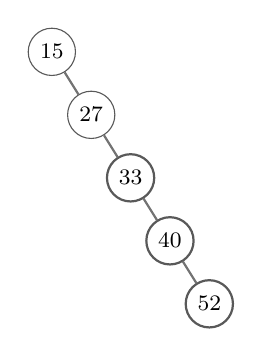
\begin{tikzpicture}[bsts, level distance=8mm,
    level 1/.style={sibling distance=10mm}, level 2/.style={sibling distance=10mm},
    level 3/.style={sibling distance=10mm}, level 4/.style={sibling distance=10mm}]
\node[bnodes] {15}
  child[missing]
  child {node {27}
    child[missing]
    child {node {33}
      child[missing]
      child {node {40}
        child[missing]
        child {node {52}}}}};
\end{tikzpicture}

{\footnotesize (a) 依 $15,\allowbreak 27,\allowbreak 33,\allowbreak 40,\allowbreak 52$ 插入，高度 $5$}
\end{minipage}\hfill
\begin{minipage}{0.45\linewidth}\centering
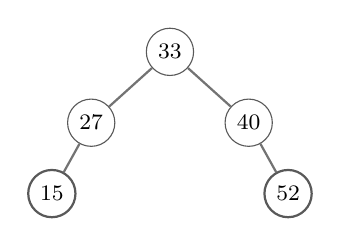
\begin{tikzpicture}[bsts, level 1/.style={sibling distance=20mm},
    level 2/.style={sibling distance=10mm}]
\node[bnodes] {33}
  child {node {27} child {node {15}} child[missing]}
  child {node {40} child[missing] child {node {52}}};
\end{tikzpicture}

{\footnotesize (b) 依 $33,\allowbreak 27,\allowbreak 40,\allowbreak 15,\allowbreak 52$ 插入，高度 $3$}
\end{minipage}
\diagcaption{同一組鍵值，插入順序不同，樹高可以差很多。}
\label{fig:bst-shapes}
\end{center}

實際的資料常常接近排好的順序：會員編號、訂單編號、時間戳記都是一直往上加的。 這正
是最壞的情況。 所以真正用在系統裡的搜尋樹，會在插入和刪除時順便調整形狀，把高度壓在
$O(\lg n)$，這是第~10~章的 AVL 樹和紅黑樹。

\subsection{隨機插入的期望高度}

如果插入順序是隨機的呢？ 說清楚一點：$n$ 個相異鍵值，$n!$ 種插入順序每一種的機率
都一樣，依這個順序插入空樹，得到的樹叫做\textbf{隨機建立的二元搜尋樹}（randomly
built binary search tree）。 結論如下，證明不在本書的範圍，延伸閱讀有出處。

\begin{theorem}
\label{thm:bst-random-height}
$n$ 個相異鍵值隨機建立的二元搜尋樹，期望高度是 $O(\lg n)$。 更精確地說，期望高度
約為 $4.311 \ln n$，大約是 $2.99 \lg n$。
\end{theorem}

為什麼會這樣？ 先看直覺。 第一個插入的鍵值當根，它在所有鍵值裡的名次是隨機的，
所以根把其餘的鍵值切成兩邊，大小是隨機的。 切得太偏（例如一邊不到四分之一）的機率大約
只有一半；每往下一層，子樹的鍵值又被隨機切一次。 一個鍵值每經過一次「切得還
算平均」的節點，它所在的子樹就縮小到原本的四分之三以下，這種事最多發生
$\log_{4/3} n$ 次，所以路徑的長度大約是 $\lg n$ 的常數倍。 這和第~14~章隨機選基準的
快速排序是同一件事：根就是第一個基準，左右子樹就是切開之後的兩堆。 如果快速排序每次
都拿子陣列裡「在插入順序中最早出現」的元素當基準，它比較過的鍵值對，和依同一個順序建
BST 時比較過的鍵值對完全相同。

高度要考慮最深的那一個節點，證明比較長。 平均深度（全部節點深度的平均）就簡單得
多，下面的框給出完整的計算，順便說明「插入順序」和「誰是誰的祖先」的關係，觀念題會
用到。

\begin{whybox}[平均深度大約是 $2 \ln n$]
把鍵值依大小編號成 $1, 2, \ldots, n$（名次）。 先看一個和機率無關的性質。

\textbf{引理。} 依某個順序把相異鍵值插入空樹。 對兩個鍵值 $i \ne j$，$i$ 是 $j$ 的
祖先，若且唯若在 $i$ 和 $j$ 之間（含兩端）的所有鍵值裡，$i$ 是最早插入的。

\textbf{證明。} 設 $I$ 是 $i$ 和 $j$ 之間（含兩端）的鍵值集合，$c$ 是 $I$ 裡最早插入
的。 在 $c$ 插入之前，樹上的節點都不在 $I$ 裡，它們每一個不是比 $I$ 的全部都小，就
是比 $I$ 的全部都大，所以 $I$ 裡的任何鍵值和它們比較，結果都一樣，往同一邊走。
因此 $I$ 的鍵值插入時都會走到 $c$ 所在的那個位置；$c$ 先到，就成為其他人的祖先。
如果 $c = i$，$i$ 就是 $j$ 的祖先。 如果 $c = j$，$j$ 是 $i$ 的祖先，$i$ 就不可能是
$j$ 的祖先。 如果 $c$ 在 $i$、$j$ 中間，$i$ 和 $j$ 到了 $c$ 會分往左右兩邊，誰也不是
誰的祖先。 \qed

隨機插入時，$I$ 有 $|i - j| + 1$ 個鍵值，每一個最早插入的機率都一樣，所以
\[
\Pr[\,i \text{ 是 } j \text{ 的祖先}\,] = \frac{1}{|i - j| + 1}.
\]
$j$ 的深度等於它的祖先個數。 用第~1~章計算插入排序平均情況時的方法（期望值的線性），
\begin{align*}
\mathrm{E}[\,j \text{ 的深度}\,]
&= \sum_{i \ne j} \frac{1}{|i - j| + 1}
= \left(\frac12 + \cdots + \frac1j\right) + \left(\frac12 + \cdots + \frac{1}{n-j+1}\right) \\
&= H_j + H_{n-j+1} - 2,
\end{align*}
其中 $H_m = 1 + \frac12 + \cdots + \frac1m$ 是第~1~章的調和數，$H_m \le \ln m + 1$。 所以每個
鍵值的期望深度都不超過 $2 \ln n$。 對 $j$ 加總，用 $\sum_{j=1}^{n} H_j = (n+1)H_n - n$，
得到全部節點的期望深度總和是 $2(n+1)H_n - 4n$，平均深度是
\[
2\left(1 + \frac1n\right) H_n - 4 \approx 2 \ln n \approx 1.39 \lg n.
\]
\end{whybox}

拿實際的數字對照：$n = 1000$ 時公式給出平均深度約 $11.0$，$n = 10^5$ 時約 $20.2$；
$n$ 變成 $100$ 倍，平均深度只多了大約 $9$。 由小到大插入時，平均深度是 $(n-1)/2$，
$n = 1000$ 時已經是 $499.5$。 用亂數洗牌建樹量出來的平均高度，$n = 1000$ 時大約
$22$、$n = 10^5$ 時大約 $41$，是 $\lg n$ 的 $2.2$ 到 $2.5$ 倍；定理說的 $2.99$ 倍是 $n$ 趨
近無限大時的比值，$n$ 不大時還有一個成長得很慢的負項把它壓低。

最後要提醒兩件事。 第一，定理只保證「插入順序隨機」時的期望值，資料本身的順序我們
通常控制不了，遇到接近排好的資料一樣會退化。 第二，定理只管插入；插入和刪除交錯很
多次之後，樹的形狀就不再是「隨機建立」的分布，沒有這麼簡單的結論。 要在任何順序下
都保證 $O(\lg n)$，就要用第~10~章的平衡樹。

\section{加上子樹大小：第 $k$ 小、排名}
\label{sec:bst-rank}

\subsection{子樹大小}

馬拉松的終點一直有人跑進來，記錄組想隨時回答兩種問題：「目前第 $k$ 快的成績是幾分
鐘？」和「完成時間 $199$ 分鐘的人目前排第幾？」 成績會不斷加入，也可能因為違規被取
消。 只用前兩節的 BST，第一個問題要做中序走訪數到第 $k$ 個，至少走過 $k$ 個節點；第二
個問題要數有幾個比它小，最壞 $\Theta(n)$。

做法是在每個節點多記一個欄位 $x.\mathit{size}$：以 $x$ 為根的子樹有幾個節點（含
$x$）。 約定 \NIL 的 $\mathit{size}$ 是 $0$，那麼對每個節點
\[
x.\mathit{size} = x.\mathit{left}.\mathit{size} + x.\mathit{right}.\mathit{size} + 1.
\]
在 $x$ 自己這棵子樹裡，比 $x$ 小的恰好是左子樹的那些節點，所以 $x$ 在子樹裡排第
$x.\mathit{left}.\mathit{size} + 1$ 小。 這個數字是下面兩個操作的關鍵。

例子：依序加入 $212,\allowbreak 187,\allowbreak 245,\allowbreak 166,\allowbreak 199,\allowbreak 230,\allowbreak 271,\allowbreak 158,\allowbreak 193,\allowbreak 238$ 這 $10$ 個完成時間
（分鐘，假設都不相同；實際上可以用「時間＋號碼布」當鍵值避免重複）。 圖中每個節點
右邊的藍色小字是 $\mathit{size}$。

\begin{center}
\begin{tikzpicture}[bst, bnode/.append style={minimum size=8.5mm},
    level 1/.style={sibling distance=56mm},
    level 2/.style={sibling distance=28mm}, level 3/.style={sibling distance=14mm}]
\node[bnode, label={[bsize]0:10}] {212}
  child {node[label={[bsize]0:5}] {187}
    child {node[label={[bsize]0:2}] {166}
      child {node[label={[bsize]0:1}] {158}}
      child[missing]}
    child {node[label={[bsize]0:2}] {199}
      child {node[label={[bsize]0:1}] {193}}
      child[missing]}}
  child {node[label={[bsize]0:4}] {245}
    child {node[label={[bsize]0:2}] {230}
      child[missing]
      child {node[label={[bsize]0:1}] {238}}}
    child {node[label={[bsize]0:1}] {271}}};
\end{tikzpicture}
\diagcaption{記了子樹大小的 BST。 由小到大是 $158,\allowbreak 166,\allowbreak 187,\allowbreak 193,\allowbreak 199,\allowbreak 212,\allowbreak 230,\allowbreak 238,\allowbreak 245,\allowbreak 271$；根 $212$ 的左子樹有 $5$ 個節點，所以 $212$ 排第 $6$。}
\label{fig:bst-size}
\end{center}

\subsection{第 $k$ 小}

從根開始，$r = x.\mathit{left}.\mathit{size} + 1$ 是 $x$ 在目前這棵子樹裡的名次。
$k = r$ 就是 $x$；$k < r$ 時答案在左子樹，仍然是第 $k$ 小；$k > r$ 時答案在右子樹，
左子樹和 $x$ 共 $r$ 個都比它小，所以在右子樹裡找第 $k - r$ 小。

\begin{pseudo}[label=alg:bst-select]{第 $k$ 小的節點（$k$ 從 $1$ 開始）}
\Function{Tree-Select}{$T, k$}
    \State $x \gets T.\mathit{root}$
    \While{$x \ne \NIL$}
        \State $r \gets x.\mathit{left}.\mathit{size} + 1$ \Comment{$x$ 在這棵子樹裡的名次}
        \If{$k = r$}
            \State \Return $x$
        \ElsIf{$k < r$}
            \State $x \gets x.\mathit{left}$
        \Else
            \State $k \gets k - r$
            \State $x \gets x.\mathit{right}$
        \EndIf
    \EndWhile
    \State \Return \NIL \Comment{$k < 1$ 或 $k$ 大於節點數}
\EndFunction
\end{pseudo}

在圖~\ref{fig:bst-size} 上找第 $7$ 小：

\begin{center}
\begin{tabular}{ccccl}
\toprule
步 & $x.\mathit{key}$ & $k$ & $r$ & 動作 \\
\midrule
1 & 212 & 7 & $5 + 1 = 6$ & $k > r$，$k \gets 7 - 6 = 1$，往右 \\
2 & 245 & 1 & $2 + 1 = 3$ & $k < r$，往左 \\
3 & 230 & 1 & $0 + 1 = 1$ & $k = r$，回傳 $230$ \\
\bottomrule
\end{tabular}
\end{center}

\subsection{排名}

反過來，給一個鍵值 $k$，問樹裡有幾個鍵值 $\le k$。 $k$ 在樹裡時，這就是 $k$ 的名
次。 從根往下搜尋 $k$，每次往右走時，$x$ 和它的左子樹都 $\le k$，把
$x.\mathit{left}.\mathit{size} + 1$ 加進答案；往左走時，$x$ 和右子樹都比 $k$ 大，不
加。

\begin{pseudo}[label=alg:bst-rank]{樹裡有幾個鍵值 $\le k$}
\Function{Tree-Rank}{$T, k$}
    \State $r \gets 0$
    \State $x \gets T.\mathit{root}$
    \While{$x \ne \NIL$}
        \If{$k < x.\mathit{key}$}
            \State $x \gets x.\mathit{left}$
        \Else \Comment{$x$ 和左子樹都 $\le k$}
            \State $r \gets r + x.\mathit{left}.\mathit{size} + 1$
            \State $x \gets x.\mathit{right}$
        \EndIf
    \EndWhile
    \State \Return $r$
\EndFunction
\end{pseudo}

這個版本找到 $k$ 之後沒有停，而是繼續往右子樹走；右子樹的鍵值都比 $k$ 大，之後只會
往左，不會再加。 這樣寫的好處是 $k$ 不在樹裡也能用。 下表是 $k = 199$ 和 $k = 240$
（不在樹裡）的過程。

\begin{center}
\begin{tabular}{ccccl}
\toprule
$k$ & $x.\mathit{key}$ & 比較 & $r$ & 說明 \\
\midrule
$199$ & 212 & $199 < 212$ & 0 & 往左 \\
      & 187 & $199 \ge 187$ & $0 + 2 + 1 = 3$ & 加上 $158, 166, 187$，往右 \\
      & 199 & $199 \ge 199$ & $3 + 1 + 1 = 5$ & 加上 $193, 199$，往右，$x = \NIL$ \\
\midrule
$240$ & 212 & $240 \ge 212$ & $0 + 5 + 1 = 6$ & 往右 \\
      & 245 & $240 < 245$ & 6 & 往左 \\
      & 230 & $240 \ge 230$ & $6 + 0 + 1 = 7$ & 往右 \\
      & 238 & $240 \ge 238$ & $7 + 0 + 1 = 8$ & 往右，$x = \NIL$ \\
\bottomrule
\end{tabular}
\end{center}

$199$ 排第 $5$，比 $240$ 分鐘快的有 $8$ 人。 兩個操作都沿著一條路徑往下走，時間
$O(h)$。 有了 \proc{Tree-Rank}，「完成時間在 $[a, b]$ 之間的有幾人」也是 $O(h)$：
用 $\le b$ 的個數減掉 $< a$ 的個數，觀念題 8 會要你寫出來。

\subsection{插入和刪除時維護 size}

$\mathit{size}$ 只有在插入和刪除時會變，而且只有\textbf{路徑上}的節點會變。

\begin{itemize}
\item \textbf{插入}：新節點的 $\mathit{size} = 1$；從根到新節點的父節點，路上每一棵
子樹都多了一個節點，各加 $1$。 在 \proc{Tree-Insert} 的第 5 行之後加上
$x.\mathit{size} \gets x.\mathit{size} + 1$ 就可以，前提是鍵值確定不在樹裡；如果可
能重複，要先搜尋一次，確定要插入了才加，否則路上的 $\mathit{size}$ 會被多加。
\item \textbf{刪除}：從根到被刪除的節點 $z$（不含 $z$），路上每一棵子樹都少一個，各減
$1$。 情況 3 時後繼 $s$ 離開原位，從 $z.\mathit{right}$ 到 $s$ 的父節點，路上的子樹也
都少了 $s$，各減 $1$；$s$ 坐到 $z$ 的位置後，它的子樹就是 $z$ 原本的子樹少掉 $z$，所
以 $s.\mathit{size} \gets z.\mathit{size} - 1$。
\end{itemize}

以圖~\ref{fig:bst-size} 取消 $187$ 為例（兩個子節點）。 從根往下找 $187$，經過的
$212$ 從 $10$ 減成 $9$。 後繼是右子樹 $\{199, 193\}$ 的最小值 $193$，從 $199$ 往左才
找到，經過的 $199$ 從 $2$ 減成 $1$。 $193$ 坐到 $187$ 的位置，$\mathit{size} = 5 - 1
= 4$。 其他節點的子樹沒有變，$\mathit{size}$ 不動。

路徑上最多 $h$ 個節點，所以多記 $\mathit{size}$ 不會讓插入和刪除變慢，仍然是
$O(h)$。 這個想法可以推廣：一個欄位只要能從「自己的資料」和「兩個子節點的同一個欄
位」算出來（例如子樹的鍵值總和、子樹的最大值），插入和刪除時就只有路徑上的節點要重
算，都能在 $O(h)$ 內維護。 反例是「節點在整棵樹裡的名次」：插入一個很小的鍵值，所有
節點的名次都加 $1$，要改 $\Theta(n)$ 個節點。 第~10~章的平衡樹會用旋轉調整形狀，到時
候還要確認旋轉時這些欄位也能在 $O(1)$ 內重算。

下面的程式依序加入那 $10$ 個成績，查第 $1, 6, 7, 11$ 快的成績，以及 $199$、$240$、
$150$ 分鐘的名次（$\le$ 它的有幾人）。 插入走兩趟：第一趟確定鍵值不在樹裡，第二趟才沿
路把 $\mathit{size}$ 加 $1$。 刪除和範例~\ref{ex:bst-member} 的 \texttt{erase} 一樣，
再照上面的規則沿路減 $1$，留給讀者練習。

\begin{example}[label=ex:bst-rank]{c}{(rank\_tree.c) 第 $k$ 快的成績與名次}
#include <stdio.h>
#include <stdlib.h>

typedef struct Node {
    int key;                    // 完成時間（分鐘），假設都不相同
    int size;                   // 以這個節點為根的子樹有幾個節點
    struct Node *left, *right;
} Node;

int size(const Node *x)
{
    return x == NULL ? 0 : x->size;
}

// 成功回傳 1，已經在樹裡回傳 0，要不到記憶體回傳 -1。
int insert(Node **root, int key)
{
    Node **link = root;                 // 第一趟：確定 key 不在樹裡
    while (*link != NULL && (*link)->key != key)
        link = key < (*link)->key ? &(*link)->left : &(*link)->right;
    if (*link != NULL)
        return 0;
    Node *z = malloc(sizeof *z);
    if (z == NULL)
        return -1;
    for (link = root; *link != NULL; ) { // 第二趟：經過的子樹都多一個
        (*link)->size++;
        link = key < (*link)->key ? &(*link)->left : &(*link)->right;
    }
    z->key = key;
    z->size = 1;
    z->left = z->right = NULL;
    *link = z;
    return 1;
}

// 第 k 小的節點（k 從 1 開始）；k 超出範圍回傳 NULL。
const Node *select_kth(const Node *x, int k)
{
    while (x != NULL) {
        int r = size(x->left) + 1;      // x 在自己這棵子樹裡排第 r
        if (k == r)
            return x;
        if (k < r) {
            x = x->left;
        } else {
            k -= r;
            x = x->right;
        }
    }
    return NULL;
}

// 樹裡有幾個鍵值 <= key。key 在樹裡時，就是它的名次。
int rank_of(const Node *x, int key)
{
    int r = 0;
    while (x != NULL) {
        if (key < x->key) {
            x = x->left;
        } else {
            r += size(x->left) + 1;     // x 和它的左子樹都 <= key
            x = x->right;
        }
    }
    return r;
}

void free_tree(Node *x)
{
    if (x == NULL)
        return;
    free_tree(x->left);
    free_tree(x->right);
    free(x);
}

int main(void)
{
    Node *root = NULL;
    int finish[] = {212, 187, 245, 166, 199, 230, 271, 158, 193, 238};
    int ks[] = {1, 6, 7, 11}, keys[] = {199, 240, 150};
    for (int i = 0; i < 10; i++)
        if (insert(&root, finish[i]) < 0)
            break;
    for (int i = 0; i < 4; i++) {
        const Node *x = select_kth(root, ks[i]);
        if (x != NULL)
            printf("kth %d: %d\n", ks[i], x->key);
        else
            printf("kth %d: none\n", ks[i]);
    }
    for (int i = 0; i < 3; i++)
        printf("rank %d: %d\n", keys[i], rank_of(root, keys[i]));
    free_tree(root);
    return 0;
}
\end{example}
\iosample{}{kth 1: 158 \\ kth 6: 212 \\ kth 7: 230 \\ kth 11: none \\ rank 199: 5 \\ rank 240: 8 \\ rank 150: 0}

\texttt{select\_kth} 和 \texttt{rank\_of} 是虛擬碼~\ref{alg:bst-select}、
\ref{alg:bst-rank} 逐行翻譯，NIL 的 $\mathit{size}$ 由函式 \texttt{size} 回傳 $0$。
$150$ 比所有成績都快，名次查詢回答 $0$，表示它插入的話會排第 $1$。

\begin{examnote}
第 $k$ 小和排名的追蹤，一步寫一列：目前的節點、$k$（或累加的 $r$）、左子樹的
$\mathit{size}$、往哪裡走。 題目只給樹、沒給 $\mathit{size}$ 時，先在每個節點旁邊標
上 $\mathit{size}$（由葉節點往上算），檢查根的 $\mathit{size}$ 等於節點總數，再開始
追蹤。
\end{examnote}

\section{本章常見錯誤}
\label{sec:bst-pitfalls}

\begin{center}
\begin{tabular}{p{0.24\linewidth}p{0.50\linewidth}p{0.16\linewidth}}
\toprule
錯誤 & 例子 & 見 \\
\midrule
只比較父子兩個節點 & 以為每個節點比左子節點大、比右子節點小就是 BST；$4$ 在 $5$
的右子樹裡卻比 $5$ 小 & 第~\ref{sec:bst-query}~節 \\
高度、深度差 1 & 題目的高度數邊（CLRS），卻套用本書數節點的公式，或反過來；把深度
和層數混用 &
第~\ref{sec:bst-query}~節 \\
以為最小值一定是葉節點 & 最小值沒有左子節點，但可能有右子樹；刪除最小值時忘了把右
子樹接回去 & 第~\ref{sec:bst-query}~節 \\
後繼只看右子樹 & 節點沒有右子樹時回答「沒有後繼」，其實後繼在祖先裡 &
第~\ref{sec:bst-query}~節 \\
插入時改到參數的複本 & \texttt{void insert(Node *root, ...)} 裡寫 \texttt{root =
malloc(...)}，呼叫端的樹沒有變 & 第~\ref{sec:bst-modify}~節 \\
遞迴刪除沒有接回子樹 & 呼叫 \texttt{erase(x->left, k)} 卻沒有寫 \texttt{x->left =}，
刪掉的節點還被指著 & 第~\ref{sec:bst-modify}~節 \\
情況 3 刪錯鍵值 & 把後繼的鍵值複製上來之後，到右子樹裡刪的還是原本的 $k$，後繼留了兩
份 & 第~\ref{sec:bst-modify}~節 \\
情況 3 找錯替代節點 & 用右子節點（而不是右子樹的最小值）取代 $z$，右子節點的左子樹
沒地方放 & 第~\ref{sec:bst-modify}~節 \\
用前序釋放 & 先 \texttt{free(x)} 再讀 \texttt{x->left} & 第~\ref{sec:bst-modify}~節 \\
把期望高度當成保證 & 以為 BST 的操作一定是 $O(\lg n)$；依序插入時是 $\Theta(n)$ &
第~\ref{sec:bst-height}~節 \\
重複鍵值時 size 多加 & 插入前沒先確定鍵值不在樹裡，沿路加了 $\mathit{size}$ 才發現重複
& 第~\ref{sec:bst-rank}~節 \\
\bottomrule
\end{tabular}
\end{center}

\section{觀念題}
\label{sec:bst-exercises}

題型和研究所考試、期中期末考的筆試相近，有選擇、計算、追蹤、證明和寫程式。 解答在
本章最後。 除非題目另外說明，鍵值都不相同，高度以節點數計算（第~7~章的定義），刪除
兩個子節點的節點時用後繼取代。

\begin{enumerate}
\item （選擇，可能不只一個答案）$T$ 是有 $n \ge 2$ 個節點的二元搜尋樹。 下列哪些敘述
一定成立？
\begin{enumerate}
\item 最小鍵值所在的節點沒有左子節點。
\item 最小鍵值所在的節點是葉節點。
\item 如果根有右子節點，根的後繼在根的右子樹裡。
\item 前序走訪的第一個鍵值是最小值。
\item 高度為 $h$ 的 BST 最少有 $h$ 個節點，最多有 $2^h - 1$ 個節點。
\end{enumerate}

\item （追蹤）依序把 $61,\allowbreak 34,\allowbreak 80,\allowbreak 12,\allowbreak 47,\allowbreak 70,\allowbreak 93,\allowbreak 25,\allowbreak 40,\allowbreak 55,\allowbreak 88,\allowbreak 43$ 插入空的二元
搜尋樹。
\begin{enumerate}
\item 畫出這棵樹，寫出它的高度和後序走訪。
\item 從 (a) 的樹刪除 $34$，分別用後繼和前驅取代，畫出兩種結果。
\item 從 (b) 用後繼的那棵樹開始，依序刪除 $80$ 和 $61$，畫出每一步之後的樹。
\end{enumerate}

\item （計算）在第 2 題 (a) 的樹上用 \proc{Iterative-Tree-Search}（虛擬碼
~\ref{alg:bst-search-iter}）搜尋整數 $k$。
\begin{enumerate}
\item 搜尋 $50$ 時依序和哪些節點比較？ 如果接著插入 $50$，它會成為哪個節點的哪一邊
子節點？
\item 哪些整數 $k$ 會在恰好和 $4$ 個節點比較之後失敗（回傳 \NIL）？ 用區間寫出答案。
\end{enumerate}

\item （計算）
\begin{enumerate}
\item 依序插入 $50,\allowbreak 30,\allowbreak 70,\allowbreak 20,\allowbreak 40,\allowbreak 60,\allowbreak 45$ 得到一棵 BST。 這 $7$ 個鍵值的 $7!$ 種
插入順序裡，有幾種會得到形狀和鍵值位置都完全相同的樹？
\item 設 $T$ 的根是 $x$，左、右子樹分別有 $a$、$b$ 個節點，能產生它們的插入順序各有
$f_L$、$f_R$ 種。 寫出能產生 $T$ 的插入順序個數，並說明理由。
\item $1, 2, \ldots, n$ 的 $n!$ 種插入順序裡，有幾種得到的樹高度是 $n$？
\end{enumerate}

\item （追蹤）在第 2 題 (a) 的樹上，每個節點加上 $\mathit{size}$。
\begin{enumerate}
\item 寫出每個節點的 $\mathit{size}$。
\item 用表格追蹤 \proc{Tree-Select}$(T, 5)$（虛擬碼~\ref{alg:bst-select}），每一步寫
出目前的節點、$k$、$r$。
\item 用表格追蹤 \proc{Tree-Rank}$(T, 50)$（虛擬碼~\ref{alg:bst-rank}）。
\end{enumerate}

\item （證明）$a < b$ 是 BST 裡的兩個鍵值，而且樹裡沒有任何鍵值介於 $a$ 和 $b$ 之間
（也就是說，排好之後它們相鄰）。 證明 $a$ 和 $b$ 所在的節點，一定有一個是另一個的祖
先。 （這裡的樹不一定只經過插入，也可能做過刪除。）

\item （證明）證明 \proc{Tree-Delete}$(x, k)$（虛擬碼~\ref{alg:bst-delete}）回傳的
樹仍然是二元搜尋樹，而且它的鍵值集合恰好是原本的集合拿掉 $k$（$k$ 不在樹裡時不
變）。 提示：對子樹的節點數做歸納。

\item （設計）$T$ 是記了 $\mathit{size}$ 的 BST，鍵值是整數。
\begin{enumerate}
\item 寫出 \proc{Tree-Floor}$(T, k)$：回傳樹裡 $\le k$ 的最大鍵值所在的節點，沒有就回
傳 \NIL。 這一小題用不到 $\mathit{size}$。
\item 利用 \proc{Tree-Rank}，在 $O(h)$ 時間內算出樹裡有幾個鍵值落在 $[a, b]$ 之間
（$a \le b$）。
\item 如果鍵值是實數，(b) 要怎麼改？
\end{enumerate}

\item （找錯）下面三個函式各有什麼錯？ 說明會發生什麼事，並改正。 \texttt{Node} 的
定義和範例~\ref{ex:bst-member} 相同。
\begin{code}{c}{觀念題 9}
// (a) 插入
void insert(Node *root, int key)
{
    if (root == NULL) {
        root = malloc(sizeof *root);
        root->key = key;
        root->left = root->right = NULL;
    } else if (key < root->key) {
        insert(root->left, key);
    } else if (key > root->key) {
        insert(root->right, key);
    }
}

// (b) 刪除，回傳子樹新的根
Node *del(Node *x, int k)
{
    if (x == NULL)
        return NULL;
    if (k < x->key) {
        x->left = del(x->left, k);
    } else if (k > x->key) {
        x->right = del(x->right, k);
    } else if (x->left == NULL || x->right == NULL) {
        Node *child = x->left != NULL ? x->left : x->right;
        free(x);
        return child;
    } else {
        Node *s = x->right;
        while (s->left != NULL)
            s = s->left;
        x->key = s->key;
        x->right = del(x->right, k);
    }
    return x;
}

// (c) 釋放整棵樹
void free_tree(Node *x)
{
    if (x == NULL)
        return;
    free(x);
    free_tree(x->left);
    free_tree(x->right);
}
\end{code}

\item （計算）隨機建立的 BST：$n$ 個鍵值的每一種插入順序機率都一樣。
\begin{enumerate}
\item $n = 3$，鍵值 $1, 2, 3$。 列出 $6$ 種順序各自得到的樹高，算出期望高度。
\item 同上，算出鍵值 $2$ 的期望深度，並和第~\ref{sec:bst-height}~節框裡的公式
$H_j + H_{n-j+1} - 2$ 比對。
\item 用同一個公式算 $n = 4$ 時鍵值 $1$ 的期望深度。
\end{enumerate}

\end{enumerate}

\section{實作練習}
\label{sec:bst-practice}

下面是 Aki-Judge 上和本章相關的題目。 「二元搜尋樹的插入與搜尋」和「二元搜尋樹的刪
除」要交函式和標頭檔，不寫 \texttt{main}；評測程式會呼叫你的插入、搜尋、刪除和中序
走訪。 「書架編號樹」只交函式，題目規定了節點的欄位名稱，重複的編號要累加本數，還要
回報那個節點的深度（根的深度是 $0$）。

\begin{center}
\begin{tabular}{llc}
\toprule
小節 & 題目 & 難度 \\
\midrule
搜尋、插入 & \akiref{bst-insert-and-search}{二元搜尋樹的插入與搜尋} & 基本 \\
搜尋、插入 & \akiref{shelf-index-tree}{書架編號樹} & 基本 \\
刪除 & \akiref{bst-deleting-keys}{二元搜尋樹的刪除} & 基本 \\
排名 & \akiref{count-keys-in-a-range-of-a-bst}{二元搜尋樹的區間計數} & 基本 \\
\bottomrule
\end{tabular}
\end{center}

「書架編號樹」的編號可能依遞增順序出現，樹會長成一條鏈，深度接近操作數；這時用遞迴
插入，遞迴深度也會跟著變大，用第~\ref{sec:bst-modify}~節的迴圈寫法比較安全。 「二元
搜尋樹的區間計數」資料量小，直接走訪就能過；也可以練習只走進可能有答案的子樹，或照觀
念題 8 加上 $\mathit{size}$。 本章的題目不多，觀念題請一定要做。

\section{讀完你應該會}
\label{sec:bst-checklist}

\begin{itemize}
\item 能依插入順序畫出 BST，寫出每次插入比較過的節點，並說出每個操作的時間是
$O(h)$。
\item 能在給定的樹上追蹤搜尋、最小／最大、後繼、前驅，分清楚「有右子樹」和「往上
找祖先」兩種情況，也會不用父指標從根往下找。
\item 能判斷刪除屬於哪一種情況，用後繼或前驅畫出刪除之後的樹，並用 \texttt{Node **}
寫出沒有特殊情況、不會漏放記憶體的 C 版插入和刪除。
\item 能說明 BST 最壞高度 $n$ 的成因，說出隨機插入的期望高度 $O(\lg n)$，並用祖
先的引理算出平均深度。
\item 能在節點加上 $\mathit{size}$，追蹤第 $k$ 小和排名，說明插入、刪除時哪些節點的
$\mathit{size}$ 要改。
\end{itemize}

\textbf{延伸閱讀}（書末會整理完整的參考資料）

\begin{itemize}
\item Thomas H. Cormen 等，\textit{Introduction to Algorithms}，第 4 版，第 12 章：
BST 的查詢、插入和刪除，刪除用另一種接指標的寫法並且維護父指標，可以和本章對照。
第 17.1 節是加上子樹大小的順序統計樹，建在紅黑樹上。 隨機建立的 BST 期望高度
$O(\lg n)$ 的完整證明在第 3 版第 12.4 節。
\item Donald E. Knuth，\textit{The Art of Computer Programming}，第 3 冊，第 6.2.2
節：二元樹搜尋的原始分析，包括隨機插入時平均比較次數的精確公式，以及刪除對樹形的影
響。
\item Steven S. Skiena，\textit{The Algorithm Design Manual}，第 3 版，第 3.4 節：
BST 的實作與「BST 到底好不好」的討論，偏重實務。
\item 《C 程式設計基礎》第~19~章：BST 的不變式、遞迴插入、三種走訪和由走訪重建，C
語法寫得比本章詳細。
\item 本書第~10~章（AVL 樹、紅黑樹）保證高度 $O(\lg n)$；第~18~章的最佳二元搜尋樹
討論已知查詢頻率時，怎麼排出平均比較次數最少的樹。
\end{itemize}

\addcontentsline{toc}{section}{觀念題解答}
\section*{觀念題解答}

\begin{enumerate}
\item (a)、(c)、(e)。 (a)：有左子節點就有更小的鍵值。 (b) 不對：最小值可以有右子
樹，例如依序插入 $1, 2$。 (c)：根有右子樹，後繼是右子樹的最小值。 (d) 不對：前序的
第一個是根，根不一定最小。 (e)：高度 $h$ 表示有 $h$ 層，從根到第 $h$ 層的某個節點
有一條 $h$ 個節點的路徑，所以至少 $h$ 個；第 $i$ 層最多 $2^{i-1}$ 個節點，
$i = 1, \ldots, h$ 加起來最多 $2^h - 1$ 個。

\item
\begin{enumerate}
\item 樹如下，高度 $5$（$61 \to 34 \to 47 \to 40 \to 43$，$5$ 個節點）。 後序走訪：$25,\allowbreak 12,\allowbreak 43,\allowbreak 40,\allowbreak 55,\allowbreak 47,\allowbreak 34,\allowbreak 70,\allowbreak 88,\allowbreak 93,\allowbreak 80,\allowbreak 61$。
\begin{center}
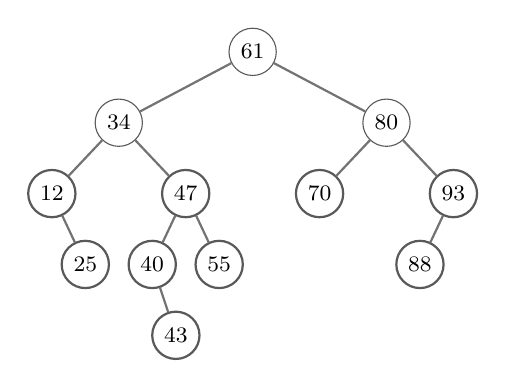
\begin{tikzpicture}[bsts]
\node[bnodes] {61}
  child {node {34}
    child {node {12} child[missing] child {node {25}}}
    child {node {47}
      child {node {40} child[missing] child {node {43}}}
      child {node {55}}}}
  child {node {80}
    child {node {70}}
    child {node {93} child {node {88}} child[missing]}};
\end{tikzpicture}
\end{center}

\item 用後繼：$34$ 的後繼是右子樹 $\{47, 40, 43, 55\}$ 的最小值 $40$。 $40$ 只有右子
節點 $43$，$43$ 頂上來成為 $47$ 的左子節點，$40$ 坐到 $34$ 的位置。 用前驅：前驅是
左子樹 $\{12, 25\}$ 的最大值 $25$，它是葉節點，直接拿下來坐到 $34$ 的位置，$12$ 的右
子節點變成 \NIL。 寫成「鍵值(左,右)」：
\begin{center}
\begin{tabular}{ll}
後繼 & $61(40(12(-,25),47(43,55)),80(70,93(88,-)))$ \\
前驅 & $61(25(12,47(40(-,43),55)),80(70,93(88,-)))$
\end{tabular}
\end{center}

\item 刪除 $80$：兩個子節點，後繼是 $93$ 子樹的最小值 $88$（葉節點），得到
$61(40(12(-,25),47(43,55)),88(70,93))$。 刪除 $61$：後繼是右子樹 $\{88, 70, 93\}$ 的
最小值 $70$（葉節點），得到 $70(40(12(-,25),47(43,55)),88(-,93))$。
\end{enumerate}

\item
\begin{enumerate}
\item $61 \to 34 \to 47 \to 55$，$50 < 55$ 往左是 \NIL，失敗。 插入 $50$ 會成為 $55$
的左子節點。
\item 失敗時比較的節點數等於「最後一個節點的深度 $+ 1$」，所以要找深度 $3$ 的節點底下
的空位。 深度 $3$ 的節點是 $25, 40, 55, 88$（$43$ 在深度 $4$）。 每個空位對應一個區
間：$25$ 的左、右是 $(12, 25)$、$(25, 34)$；$40$ 的左是 $(34, 40)$（右邊有 $43$）；
$55$ 的左、右是 $(47, 55)$、$(55, 61)$；$88$ 的左、右是 $(80, 88)$、$(88, 93)$。
整數答案：$13 \sim 24$、$26 \sim 33$、$35 \sim 39$、$48 \sim 54$、$56 \sim 60$、
$81 \sim 87$、$89 \sim 92$。
\end{enumerate}

\item
\begin{enumerate}
\item 樹是 $50(30(20,40(-,45)),70(60,-))$。 用 (b) 的公式：$50$ 必須第一個插入；左子
樹 $\{30, 20, 40, 45\}$ 和右子樹 $\{70, 60\}$ 的插入順序可以任意交錯。 左子樹裡 $30$
最先，接著 $\{20\}$ 和 $\{40, 45\}$ 交錯，$40$ 要在 $45$ 前面：$\binom{3}{1} \cdot 1
\cdot 1 = 3$ 種。 右子樹只能 $70, 60$：$1$ 種。 合計 $\binom{6}{4} \cdot 3 \cdot 1 =
45$ 種。
\item $\binom{a+b}{a} f_L f_R$。 根必須最先插入，否則先插入的那個鍵值會成為根。 之後
左子樹的鍵值插入時一定走到根的左邊，只和左子樹的其他鍵值互相影響；右子樹也一樣。 所
以一個插入順序產生 $T$，若且唯若根在最前面，而且把它拆成「左子樹的鍵值」和「右子樹
的鍵值」兩個子序列時，各自產生左、右子樹。 左右兩個子序列各有 $f_L$、$f_R$ 種，在
後面 $a + b$ 個位置裡，選 $a$ 個位置放左子樹的鍵值，有 $\binom{a+b}{a}$ 種選法。
\item 高度 $n$ 表示 $n$ 層各一個節點，每個節點最多一個子節點，樹是一條鏈。 這時每一
步插入的都必須是剩下的鍵值裡最小或最大的那個，否則剩下的鍵值會分到它的兩邊。 前
$n - 1$ 步各有 $2$ 種選擇，最後一步只剩一個，共 $2^{n-1}$ 種。 例如 $n = 7$ 時是 $64$ 種。
\end{enumerate}

\item
\begin{enumerate}
\item 葉節點 $25,\allowbreak 43,\allowbreak 55,\allowbreak 70,\allowbreak 88$ 都是 $1$；$12$：$2$；$40$：$2$；$47$：$4$；$34$：
$7$；$93$：$2$；$80$：$4$；$61$：$12$。
\item
\begin{tabular}[t]{ccccl}
\toprule
步 & $x.\mathit{key}$ & $k$ & $r$ & 動作 \\
\midrule
1 & 61 & 5 & $7 + 1 = 8$ & $k < r$，往左 \\
2 & 34 & 5 & $2 + 1 = 3$ & $k > r$，$k \gets 2$，往右 \\
3 & 47 & 2 & $2 + 1 = 3$ & $k < r$，往左 \\
4 & 40 & 2 & $0 + 1 = 1$ & $k > r$，$k \gets 1$，往右 \\
5 & 43 & 1 & $0 + 1 = 1$ & $k = r$，回傳 $43$ \\
\bottomrule
\end{tabular}

第 $5$ 小是 $43$（由小到大：$12,\allowbreak 25,\allowbreak 34,\allowbreak 40,\allowbreak 43,\allowbreak \ldots$）。
\item
\begin{tabular}[t]{cccl}
\toprule
$x.\mathit{key}$ & 比較 & $r$ & 動作 \\
\midrule
61 & $50 < 61$ & 0 & 往左 \\
34 & $50 \ge 34$ & $0 + 2 + 1 = 3$ & 往右 \\
47 & $50 \ge 47$ & $3 + 2 + 1 = 6$ & 往右 \\
55 & $50 < 55$ & 6 & 往左，$x = \NIL$ \\
\bottomrule
\end{tabular}

回傳 $6$：$\le 50$ 的有 $12,\allowbreak 25,\allowbreak 34,\allowbreak 40,\allowbreak 43,\allowbreak 47$。
\end{enumerate}

\item 設 $c$ 是 $a$ 和 $b$ 的最低共同祖先（同時是兩者祖先的節點裡最深的那個；節點也
算自己的祖先）。 如果 $c$ 就是 $a$ 或 $b$，結論成立。 否則 $a$ 和 $b$ 不可能在 $c$
的同一棵子樹裡（不然 $c$ 的那個子節點也是共同祖先，比 $c$ 深），所以一個在左子樹、一
個在右子樹。 由 BST 性質，左邊的比 $c.\mathit{key}$ 小，右邊的比 $c.\mathit{key}$
大，而 $a < b$，所以 $a < c.\mathit{key} < b$，和「沒有鍵值介於 $a$、$b$ 之間」矛
盾。 證明只用到 BST 性質，和樹是怎麼來的無關，所以做過刪除也成立。

\item 對 $x$ 這棵子樹的節點數 $m$ 做歸納，證明：如果 $x$ 是一棵 BST，
\proc{Tree-Delete}$(x, k)$ 回傳一棵 BST，鍵值集合是原本的集合拿掉 $k$。

$m = 0$：$x = \NIL$，回傳 \NIL，成立。

$m \ge 1$，分情況。 (i) $k < x.\mathit{key}$：由歸納假設，第 5 行之後左子樹是 BST，
鍵值是原本的左子樹拿掉 $k$，仍然都比 $x.\mathit{key}$ 小；右子樹沒動；所以整棵仍是
BST，鍵值少了 $k$（$k$ 不在樹裡時不變）。 (ii) $k > x.\mathit{key}$：對稱。
(iii) $k = x.\mathit{key}$ 而且至少一個子樹是空的（第 8 到 11 行）：回傳另一棵子樹，
它本來就是 BST，鍵值恰好是原本的集合拿掉 $k$。 (iv) 兩個子樹都不空：$s$ 是右子樹的
最小值。 第 14 行之後 $x.\mathit{key} = s.\mathit{key}$；由歸納假設，第 15 行之後右
子樹是 BST，鍵值是原本的右子樹拿掉 $s.\mathit{key}$，剩下的都比 $s.\mathit{key}$
大。 左子樹的鍵值都比原本的 $k$ 小，而 $k < s.\mathit{key}$，所以也都比新的
$x.\mathit{key}$ 小。 因此 $x$ 仍滿足 BST 性質。 鍵值集合：$k$ 被 $s.\mathit{key}$
蓋掉，右子樹少了一份 $s.\mathit{key}$，合起來恰好少了 $k$。

\item
\begin{enumerate}
\item 和 \proc{Successor-Of-Key} 對稱，往右走時記下候選：
\begin{pseudo}{觀念題 8 的解答}
\Function{Tree-Floor}{$T, k$}
    \State $f \gets \NIL$
    \State $x \gets T.\mathit{root}$
    \While{$x \ne \NIL$}
        \If{$x.\mathit{key} = k$}
            \State \Return $x$
        \ElsIf{$x.\mathit{key} < k$}
            \State $f \gets x$ \Comment{$x$ 是目前 $\le k$ 的最大候選}
            \State $x \gets x.\mathit{right}$
        \Else
            \State $x \gets x.\mathit{left}$
        \EndIf
    \EndWhile
    \State \Return $f$
\EndFunction
\end{pseudo}
只走一條路徑，$O(h)$。
\item 答案是 $\proc{Tree-Rank}(T, b) - \proc{Tree-Rank}(T, a - 1)$：前者是 $\le b$ 的
個數，後者是 $\le a - 1$，也就是 $< a$ 的個數（鍵值是整數）。 兩次各 $O(h)$。
\item 實數沒有「$a - 1$」可以用。 改成 $\proc{Tree-Rank}(T, b) - \proc{Tree-Rank}(T,
a)$，如果 $a$ 在樹裡（用 \proc{Tree-Search} 查，$O(h)$），再加 $1$。 也可以另外寫一個
「$< k$ 的個數」，把 \proc{Tree-Rank} 第 5 行的 $k < x.\mathit{key}$ 改成 $k \le
x.\mathit{key}$。
\end{enumerate}

\item
(a) \texttt{root} 是參數的複本。 樹是空的時，\texttt{malloc} 來的節點只存在函式裡，
回到呼叫端時樹還是空的，而且那塊記憶體再也沒人指著（洩漏）。 遞迴到
\texttt{root->left == NULL} 時也一樣，新節點沒有接上。 改法：收 \texttt{Node **}，寫
\texttt{*root = ...}；或回傳子樹的根，呼叫端寫 \texttt{root->left = insert(root->left,
key)}。

(b) 兩個子節點時，把後繼的鍵值複製到 \texttt{x} 之後，到右子樹刪的還是 \texttt{k}。
\texttt{k} 比右子樹的每個鍵值都小，什麼也刪不到，結果是後繼的鍵值出現兩次，\texttt{k}
卻消失了（而且沒有任何節點被釋放）。 改成 \texttt{x->right = del(x->right, x->key);}
（此時 \texttt{x->key} 就是後繼的鍵值）。 其他部分是對的：只有一個子節點或沒有子節點
時，\texttt{child} 是那個子節點或 \texttt{NULL}。

(c) \texttt{free(x)} 之後又讀 \texttt{x->left}、\texttt{x->right}，是讀已經釋放的記憶
體。 改成後序：先遞迴釋放兩棵子樹，最後才 \texttt{free(x)}。

\item
\begin{enumerate}
\item $2$ 先插入的兩種順序（$2, 1, 3$ 和 $2, 3, 1$）得到高度 $2$；其他四種（$1$ 或 $3$
先插入）都是一條鏈，高度 $3$。 期望高度 $(2 \cdot 2 + 4 \cdot 3)/6 = 8/3$。
\item $2$ 最先插入時深度 $0$（$2$ 種）。 $1, 2, 3$ 和 $3, 2, 1$ 時深度 $1$；$1, 3, 2$
和 $3, 1, 2$ 時深度 $2$。 期望深度 $(0 + 0 + 1 + 1 + 2 + 2)/6 = 1$。 公式：$j = 2$，
$n = 3$，$H_2 + H_2 - 2 = \frac32 + \frac32 - 2 = 1$，相同。
\item $j = 1$，$n = 4$：$H_1 + H_4 - 2 = 1 + \frac{25}{12} - 2 = \frac{13}{12}$。
\end{enumerate}

\end{enumerate}
